\documentclass[portrait,a0paper,fontscale=0.277]{baposter}

\usepackage{calc}
\usepackage{graphicx}
\usepackage{amsmath}
\usepackage{amssymb}
\usepackage{relsize}
\usepackage{multirow}
\usepackage{rotating}
\usepackage{bm}
\usepackage{url}
\usepackage{txfonts}

%\usepackage{wrapfig}

\usepackage{graphicx}
\usepackage{multicol}

%\usepackage{times}
%\usepackage{helvet}
%\usepackage{bookman}
\usepackage{palatino}

\newcommand{\captionfont}{\footnotesize}

\graphicspath{{images/}{../images/}}
\usetikzlibrary{calc}

\newcommand{\SET}[1]  {\ensuremath{\mathcal{#1}}}
\newcommand{\MAT}[1]  {\ensuremath{\boldsymbol{#1}}}
\newcommand{\VEC}[1]  {\ensuremath{\boldsymbol{#1}}}
\newcommand{\Video}{\SET{V}}
\newcommand{\video}{\VEC{f}}
\newcommand{\track}{x}
\newcommand{\Track}{\SET T}
\newcommand{\LMs}{\SET L}
\newcommand{\lm}{l}
\newcommand{\PosE}{\SET P}
\newcommand{\posE}{\VEC p}
\newcommand{\negE}{\VEC n}
\newcommand{\NegE}{\SET N}
\newcommand{\Occluded}{\SET O}
\newcommand{\occluded}{o}


% New definition of square root:
% it renames \sqrt as \oldsqrt
\let\oldsqrt\sqrt
% it defines the new \sqrt in terms of the old one
\def\sqrt{\mathpalette\DHLhksqrt}
\def\DHLhksqrt#1#2{%
\setbox0=\hbox{$#1\oldsqrt{#2\,}$}\dimen0=\ht0
\advance\dimen0-0.2\ht0
\setbox2=\hbox{\vrule height\ht0 depth -\dimen0}%
{\box0\lower0.4pt\box2}}

%%%%%%%%%%%%%%%%%%%%%%%%%%%%%%%%%%%%%%%%%%%%%%%%%%%%%%%%%%%%%%%%%%%%%%%%%%%%%%%%
%%%% Some math symbols used in the text
%%%%%%%%%%%%%%%%%%%%%%%%%%%%%%%%%%%%%%%%%%%%%%%%%%%%%%%%%%%%%%%%%%%%%%%%%%%%%%%%

%%%%%%%%%%%%%%%%%%%%%%%%%%%%%%%%%%%%%%%%%%%%%%%%%%%%%%%%%%%%%%%%%%%%%%%%%%%%%%%%
% Multicol Settings
%%%%%%%%%%%%%%%%%%%%%%%%%%%%%%%%%%%%%%%%%%%%%%%%%%%%%%%%%%%%%%%%%%%%%%%%%%%%%%%%
\setlength{\columnsep}{1.5em}
\setlength{\columnseprule}{0mm}

%%%%%%%%%%%%%%%%%%%%%%%%%%%%%%%%%%%%%%%%%%%%%%%%%%%%%%%%%%%%%%%%%%%%%%%%%%%%%%%%
% Save space in lists. Use this after the opening of the list
%%%%%%%%%%%%%%%%%%%%%%%%%%%%%%%%%%%%%%%%%%%%%%%%%%%%%%%%%%%%%%%%%%%%%%%%%%%%%%%%
\newcommand{\compresslist}{%
\setlength{\itemsep}{1pt}%
\setlength{\parskip}{0pt}%
\setlength{\parsep}{0pt}%
}

%%%%%%%%%%%%%%%%%%%%%%%%%%%%%%%%%%%%%%%%%%%%%%%%%%%%%%%%%%%%%%%%%%%%%%%%%%%%%%
%%% Begin of Document
%%%%%%%%%%%%%%%%%%%%%%%%%%%%%%%%%%%%%%%%%%%%%%%%%%%%%%%%%%%%%%%%%%%%%%%%%%%%%%

\begin{document}

%%%%%%%%%%%%%%%%%%%%%%%%%%%%%%%%%%%%%%%%%%%%%%%%%%%%%%%%%%%%%%%%%%%%%%%%%%%%%%
%%% Here starts the poster
%%%---------------------------------------------------------------------------
%%% Format it to your taste with the options
%%%%%%%%%%%%%%%%%%%%%%%%%%%%%%%%%%%%%%%%%%%%%%%%%%%%%%%%%%%%%%%%%%%%%%%%%%%%%%
% Define some colors

%\definecolor{lightblue}{cmyk}{0.83,0.24,0,0.12}
\definecolor{lightblue}{rgb}{0.145,0.6666,1}

% Draw a video
\newlength{\FSZ}
\newcommand{\drawvideo}[3]{% [0 0.25 0.5 0.75 1 1.25 1.5]
   \noindent\pgfmathsetlength{\FSZ}{\linewidth/#2}
   \begin{tikzpicture}[outer sep=0pt,inner sep=0pt,x=\FSZ,y=\FSZ]
   \draw[color=lightblue!50!black] (0,0) node[outer sep=0pt,inner sep=0pt,text width=\linewidth,minimum height=0] (video) {\noindent#3};
   \path [fill=lightblue!50!black,line width=0pt] 
     (video.north west) rectangle ([yshift=\FSZ] video.north east) 
    \foreach \x in {1,2,...,#2} {
      {[rounded corners=0.6] ($(video.north west)+(-0.7,0.8)+(\x,0)$) rectangle +(0.4,-0.6)}
    }
;
   \path [fill=lightblue!50!black,line width=0pt] 
     ([yshift=-1\FSZ] video.south west) rectangle (video.south east) 
    \foreach \x in {1,2,...,#2} {
      {[rounded corners=0.6] ($(video.south west)+(-0.7,-0.2)+(\x,0)$) rectangle +(0.4,-0.6)}
    }
;
   \foreach \x in {1,...,#1} {
     \draw[color=lightblue!50!black] ([xshift=\x\linewidth/#1] video.north west) -- ([xshift=\x\linewidth/#1] video.south west);
   }
   \foreach \x in {0,#1} {
     \draw[color=lightblue!50!black] ([xshift=\x\linewidth/#1,yshift=1\FSZ] video.north west) -- ([xshift=\x\linewidth/#1,yshift=-1\FSZ] video.south west);
   }
   \end{tikzpicture}
}

\hyphenation{resolution occlusions}
%%
\begin{poster}%
  % Poster Options
  {
  % Show grid to help with alignment
  grid=false,
  % Column spacing
  colspacing=1em,
  % Color style
  bgColorOne=white,
  bgColorTwo=white,
  borderColor=lightblue,
  headerColorOne=black,
  headerColorTwo=lightblue,
  headerFontColor=white,
  boxColorOne=white,
  boxColorTwo=lightblue,
  % Format of textbox
  textborder=roundedleft,
  % Format of text header
  eyecatcher=true,
  headerborder=closed,
  headerheight=0.14\textheight,
%  textfont=\sc, An example of changing the text font
  headershape=roundedright,
  headershade=shadelr,
  headerfont=\normalsize\bf\textsc, %Sans Serif
  textfont={\setlength{\parindent}{1.5em}},
  boxshade=plain,
%  background=shade-tb,
  background=plain,
  linewidth=2pt
  }
  % Eye Catcher
  {
\includegraphics[height=8.5em]{images/logo1}} 
  % Title
  {\bf\Large{Dynamics of photo-excited Ba$^+$ cations in helium nanodroplets}\vspace{0.5em}}
  % Authors
  {\normalsize{ \underline{A. Leal},$^1$ M.Barranco,$^1$ F. Cargnoni,$^2$ M. Drabbels,$^3$ A. Hernando,$^4$ D. Mateo,$^1$ M. Mella,$^5$ M. Pi$^1$\vspace{0.5em}} \\
\smaller{$^1$Departament E.C.M., Facultat de F\'isica, and IN$^2$UB, Universitat de Barcelona, Diagonal 645, E-08028 Barcelona, Spain 
\\ \vspace{2px}
$^2$Instituto di Scienze e Tecnologie Molecolari (ISTM), Consiglio Nazionale delle Ricerche, 
via Golgi 19, 20133 Milano, Italy
\\ \vspace{2px}
$^3$Laboratoire de Chimie Physique Moleculaire, Swiss Federal Institute of Lausanne (EPFL),
CH-1015 Lausanne, Switzerland
\\ \vspace{2px}
$^4$Laboratory of Theoretical Physical Chemistry, Institut des Sciences et Ingenierie Chimiques,\\
Swiss Federal Institute of Technology Lausanne (EPFL), CH-1015 Lausanne, Switzerland
\\ \vspace{2px}
$^5$Dipartimento di Scienza ed Alta Tecnologia, Universita degli Studi dell'Insubria, via Valleggio 11,
22100 Como, Italy

}}
  % University logo
  {% The makebox allows the title to flow into the logo, this is a hack because of the L shaped logo.
   
\includegraphics[height=8.5em]{images/logo2}
  }

%%%%%%%%%%%%%%%%%%%%%%%%%%%%%%%%%%%%%%%%%%%%%%%%%%%%%%%%%%%%%%%%%%%%%%%%%%%%%%
%%% Now define the boxes that make up the poster
%%%---------------------------------------------------------------------------
%%% Each box has a name and can be placed absolutely or relatively.
%%% The only inconvenience is that you can only specify a relative position 
%%% towards an already declared box. So if you have a box attached to the 
%%% bottom, one to the top and a third one which should be in between, you 
%%% have to specify the top and bottom boxes before you specify the middle 
%%% box.
%%%%%%%%%%%%%%%%%%%%%%%%%%%%%%%%%%%%%%%%%%%%%%%%%%%%%%%%%%%%%%%%%%%%%%%%%%%%%%
    %
    % A coloured circle useful as a bullet with an adjustably strong filling
    \newcommand{\colouredcircle}{%
      \tikz{\useasboundingbox (-0.2em,-0.32em) rectangle(0.2em,0.32em); \draw[draw=black,fill=lightblue,line width=0.03em] (0,0) circle(0.18em);}}

%%%%%%%%%%%%%%%%%%%%%%%%%%%%%%%%%%%%%%%%%%%%%%%%%%%%%%%%%%%%%%%%%%%%%%%%%%%%%%
  \headerbox{Abstract}{name=abstract,column=0,row=0,span=3}{
%%%%%%%%%%%%%%%%%%%%%%%%%%%%%%%%%%%%%%%%%%%%%%%%%%%%%%%%%%%%%%%%%%%%%%%%%%%%%%
\vspace{2px}  
\scriptsize{
\noindent Within TDDFT, we have addressed the dynamics of Ba$^+$ cations in helium nanodroplets. The absorption spectra from S to P and D states, as well as the emission spectra from P to S and D states of the cation are discussed. The appearance of exciplexes is discussed and the dynamics of the excited Ba$^+$ cation in the P state has been investigated.
}

\vspace{2px}
 }

%%%%%%%%%%%%%%%%%%%%%%%%%%%%%%%%%%%%%%%%%%%%%%%%%%%%%%%%%%%%%%%%%%%%%%%%%%%%%%
  \headerbox{Potentials}{name=potentials,column=0,row=0,span=1, below=abstract}{
%%%%%%%%%%%%%%%%%%%%%%%%%%%%%%%%%%%%%%%%%%%%%%%%%%%%%%%%%%%%%%%%%%%%%%%%%%%%%%
\vspace{2px}  
\scriptsize{

\noindent For the $^2$P states, the pair potentials have been written as a direction-dependent combination of $\Pi$ and $\Sigma$ potentials

\begin{equation*}
	V_{\lambda}(\textbf{r}) = \langle\lambda\vert V(r)\vert\lambda\rangle = \sum_{ijss'}\lambda_{is}^{*}{\cal V}^{ijss'}(\textbf{r})\lambda_{js'},
\end{equation*}

\noindent where the six-dimentional matrix operator V has components

\begin{equation*}
	{\cal V}^{ijss'}(\textbf{r}) = \left[V_\Pi(r)\delta_{ij}+\left(V_\Sigma(r)-V_\Pi(r)\right)\frac{r_ir_j}{r^2}\right]\delta_{ss'}.
\end{equation*}

\begin{center}
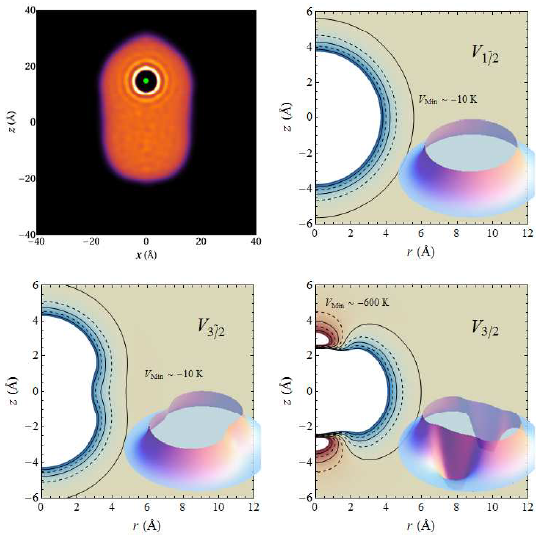
\includegraphics[width=0.87\linewidth]{Ppotential}\\

\vspace{5px}
\end{center}

\noindent Using a generalization of the method above, the corresponding potentials for the $^2$D states can be obtained

\begin{center}
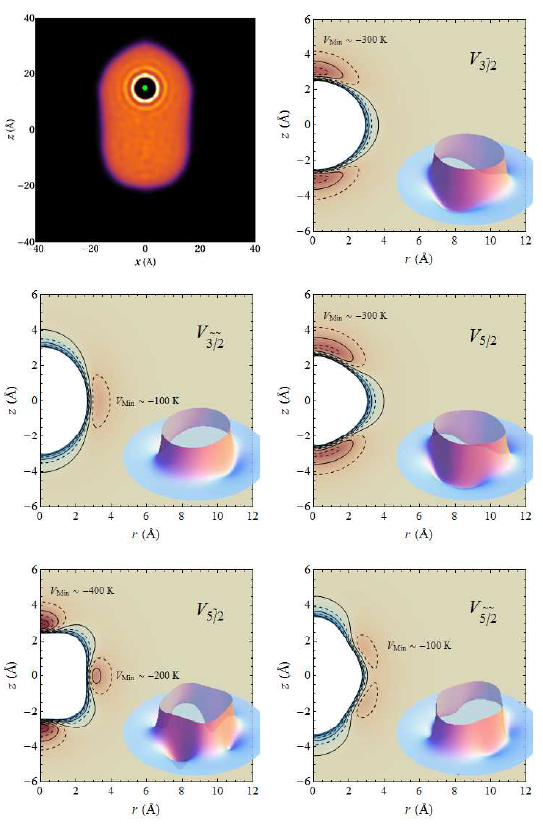
\includegraphics[width=0.87\linewidth]{Dpotential}\\
\end{center}
}

\noindent For both cases, the density used to calculate the potentials is the one showed in the top-left panel of each figure, corresponding to a turning point of the neutral Ba$^+$ dynamics.

\vspace{2px}
 }
 
%%%%%%%%%%%%%%%%%%%%%%%%%%%%%%%%%%%%%%%%%%%%%%%%%%%%%%%%%%%%%%%%%%%%%%%%%%%%%%
  \headerbox{DFT Framework $^{[1]}$}{name=DFT,column=1,row=0,span=2, below=abstract}{
%%%%%%%%%%%%%%%%%%%%%%%%%%%%%%%%%%%%%%%%%%%%%%%%%%%%%%%%%%%%%%%%%%%%%%%%%%%%%%
\vspace{2px}  
\scriptsize{
\noindent The dynamic evolution of the electronic excited state of Ba$^+$ is described introducing an additional degree of freedom, a six-component vector $\vert\lambda\rangle$ written in terms of same basis for spin and angular momentum used for the SO interaction.

\begin{equation*}
\vert\lambda\rangle=\sum_{is}\lambda_{is}(i,s)
\end{equation*}

\noindent The total energy of the Ba$^+$@$^4$He$_{1000}$ complex suddenly excited to the $^2$P manifold is written as

\begin{equation*}
	E\left[\Psi,r_{Ba^+},\lambda\right]=\int dr \frac{\hbar^2}{2m_{He}}\vert\nabla\Psi\vert^2+\frac{p^2_{Ba^+}}{2m_{Ba^+}}
	+\int dr \varepsilon_{He}\left[\rho\right]+\langle\lambda\vert V_{SO}\vert\lambda\rangle+\int dr\rho(r)V_\lambda\left(r-r_{Ba^+}\right)
\end{equation*}

\noindent The following coupled 3D time-dependent system, resulting from the variation of the action, has to be solved to obtain the dynamical evolution

\begin{equation*}
	i\hbar\frac{\partial}{\partial t}\Psi_{He}=\left[-\frac{\hbar^2}{2m_{He}}\nabla^2+\frac{\delta\varepsilon_{He}}{\delta\rho(r)}
	+V_\lambda\left(r-r_{Ba^+}\right)\right]\Psi_{He} \;\;\;\;\;\;\;\;\;\;\;\;\; , \;\;\;\;\;\;\;\;\;\;\;\;\; i\hbar\frac{\partial}{\partial t}\vert\lambda\rangle={\cal H}\vert\lambda\rangle
\end{equation*}

\begin{equation*}
	m_{Ba^+}\ddot{r}_{Ba^+}=-\nabla_{r_{Ba^+}}\left[\int dr\rho(r)V_\lambda\left(r-r_{Ba^+}\right)\right]=
	-\int dr\nabla\rho(r)V_\lambda\left(r-r_{Ba^+}\right)
\end{equation*}

\noindent The electronic state Hamiltonian ${\cal H}$ is a 6$\times$6 matrix whose elements are given by
\begin{equation*}
	H^{ijss'}=\int dr\rho(r){\cal V}^{ijss'}\left(r-r_{Ba^+_0}\right)+V^{ijss'}_{SO}
\end{equation*}
}
\vspace{-10px}
 }
 
%%%%%%%%%%%%%%%%%%%%%%%%%%%%%%%%%%%%%%%%%%%%%%%%%%%%%%%%%%%%%%%%%%%%%%%%%%%%%%
  \headerbox{$^2$P$_{1/2}$ Dynamics}{name=dynamics,column=1,row=0,span=2, below=DFT}{
%%%%%%%%%%%%%%%%%%%%%%%%%%%%%%%%%%%%%%%%%%%%%%%%%%%%%%%%%%%%%%%%%%%%%%%%%%%%%%
\vspace{2px}  
\scriptsize{
\noindent To solve the above equations initial values for the variables are required.
We have chosen as starting configuration that corresponding to the turning
point reached by the Ba$^+$ in the ground state 223 ps after the ionization of
neutral Ba in the surface dimple state.$^{[2]}$
\begin{center}
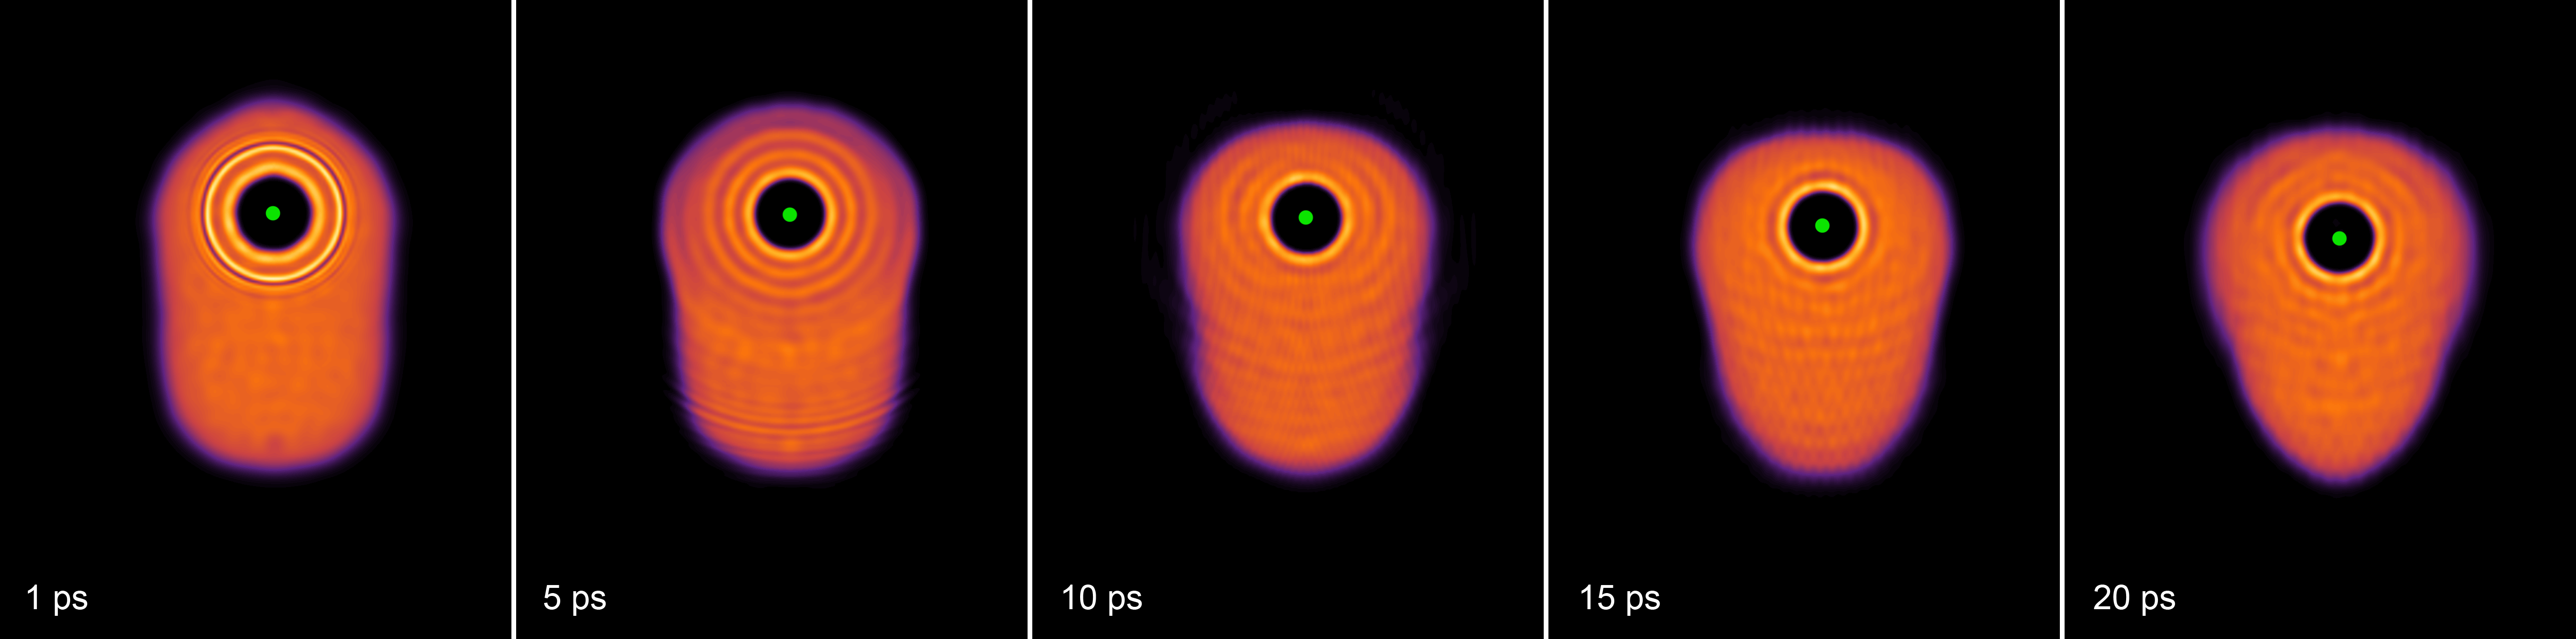
\includegraphics[width=0.82\linewidth]{return}\\
\end{center}

\noindent We have also followed the dynamic evolution of some particular configurations, like a metastable stretched configuration corresponding to $z_0 = 44.6 \AA$.
\begin{center}
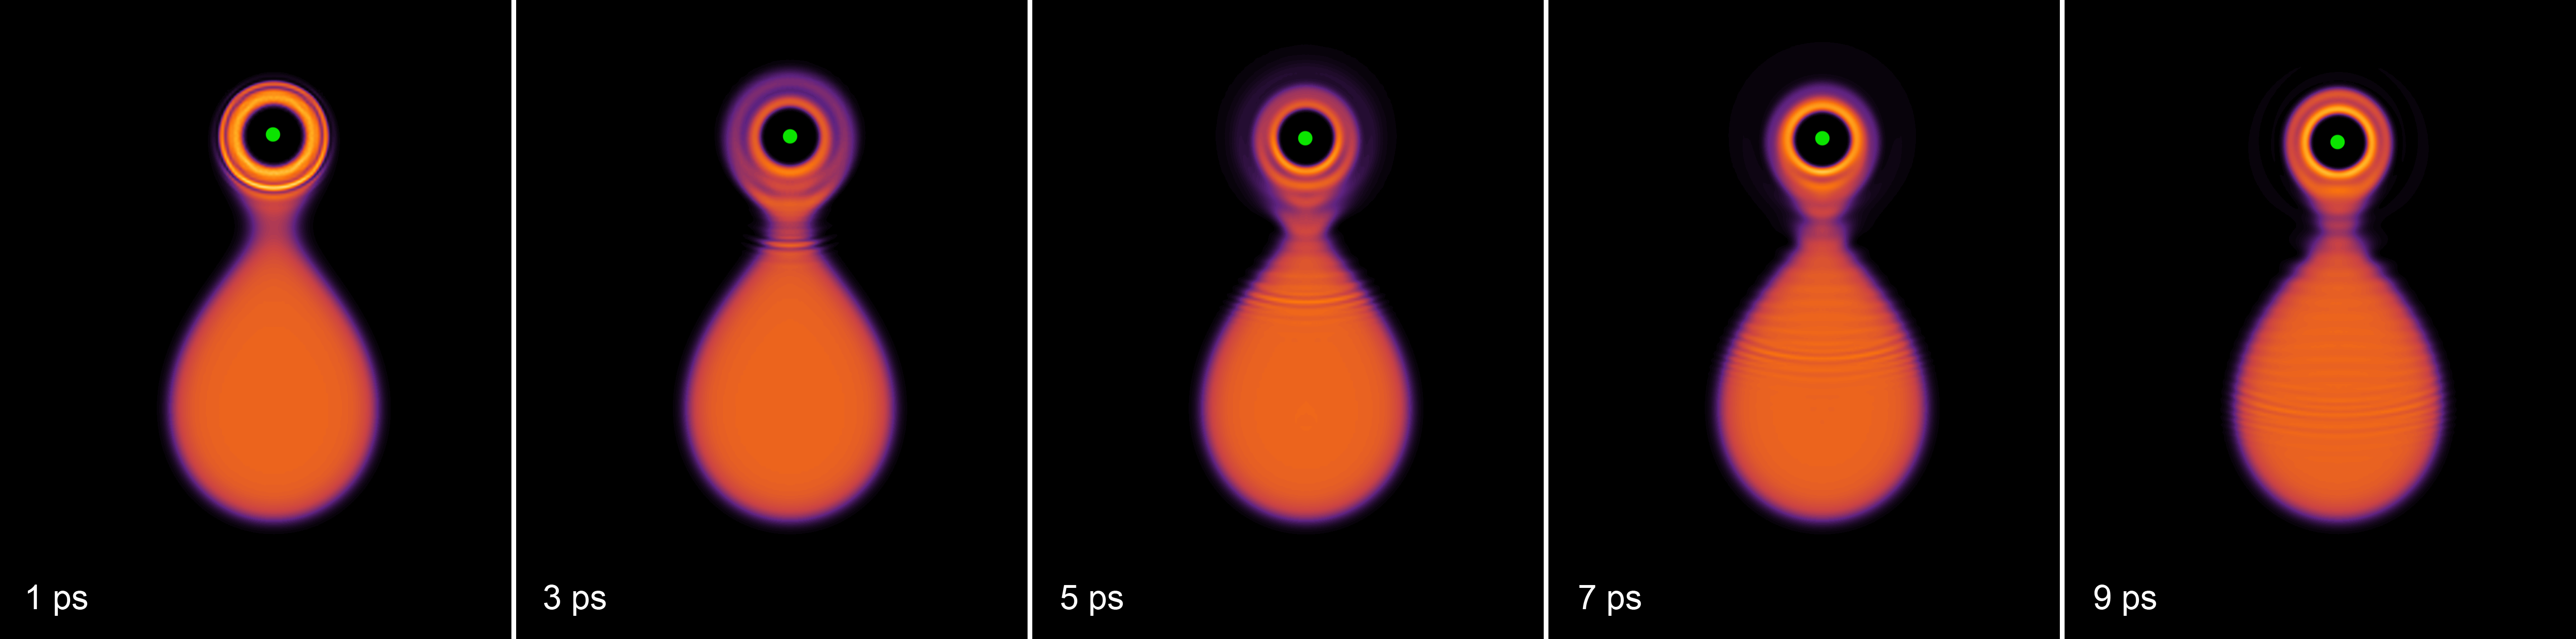
\includegraphics[width=0.82\linewidth]{stretched}\\
\end{center}
}

\vspace{2px}
 }
 
 
 
%%%%%%%%%%%%%%%%%%%%%%%%%%%%%%%%%%%%%%%%%%%%%%%%%%%%%%%%%%%%%%%%%%%%%%%%%%%%%%
  \headerbox{Absorption spectrum and preliminary results on emission spectra}{name=spectra,column=1,span=2, below=dynamics, above=bottom}{
%%%%%%%%%%%%%%%%%%%%%%%%%%%%%%%%%%%%%%%%%%%%%%%%%%%%%%%%%%%%%%%%%%%%%%%%%%%%%%
\vspace{2px}  
\scriptsize{
\noindent We have calculated the absorption and emission spectra of Ba$^+$ between the ground state and $^2$P and $^2$D manifolds. The absorption spectrum and some preliminary results on the emission spectra are shown in the figure below.

\begin{center}
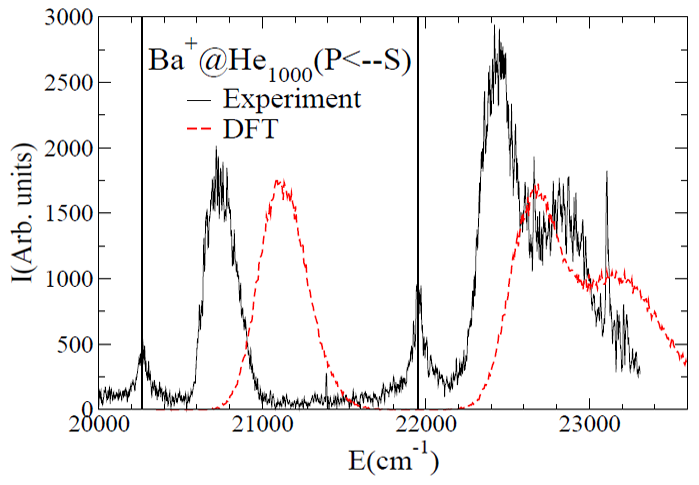
\includegraphics[width=0.33\linewidth]{absSP2}
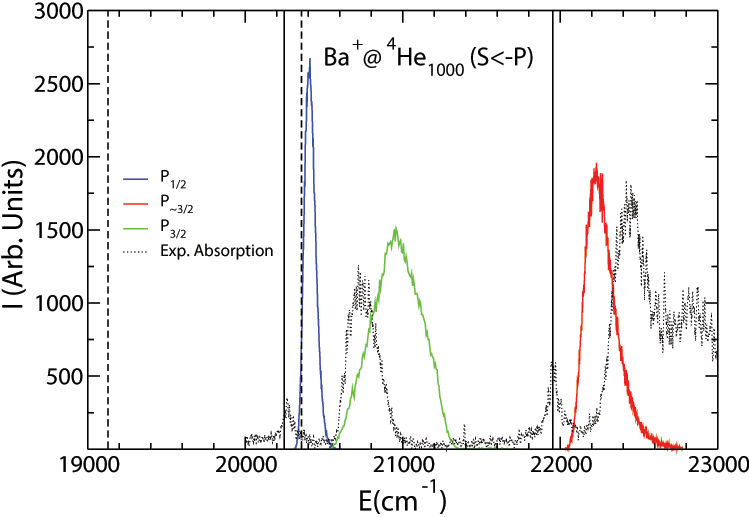
\includegraphics[width=0.33\linewidth]{emission}
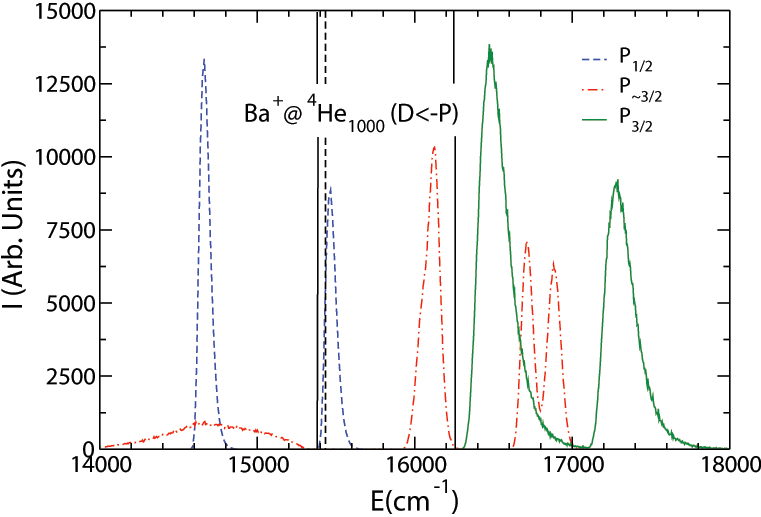
\includegraphics[width=0.33\linewidth]{PD}
\end{center}
}

\noindent In the absorption spectrum (left panel) the dashed line corresponds to the calculated spectrum while the solid one shows the experimental results. The center panel shows the S $\longleftarrow$ P emission spectrum, where the coloured solid lines represents the emission lines and in order to compare, the dotted one shows the experimental absorption spectrum. The D $\longleftarrow$ P emission spectrum is shown in the right panel. In the three panels, the vertical solid lines represent the persistent lines of singly ionized barium in the gas phase and the vertical dashed lines indicate the experimental peaks found in this energy region.$^{[3]}$

\vspace{2px}
 }
 

%%%%%%%%%%%%%%%%%%%%%%%%%%%%%%%%%%%%%%%%%%%%%%%%%%%%%%%%%%%%%%%%%%%%%%%%%%%%%%
  \headerbox{References}{name=references,column=0,span=1, below=potentials, above=bottom}{
%%%%%%%%%%%%%%%%%%%%%%%%%%%%%%%%%%%%%%%%%%%%%%%%%%%%%%%%%%%%%%%%%%%%%%%%%%%%%%
\vspace{2px}  
\scriptsize{ \vspace{2px}
\noindent [1] D. Mateo et al., PCCP \textbf{15}, 18388-18400 (2013) \\ 
\\
\noindent [2] D. Mateo et al., J. Chem. Phys. \textbf{140}, 131101 (2014)\\ 
\\
\noindent [3] H.J. Reyher et al. Phys. Lett. A \textbf{115}, 238 (1986). \\ 
}

\vspace{2px}
 }

 
\end{poster}

\end{document}

